%!TEX root = ../thesis.tex
%*******************************************************************************
%****************************** Third Chapter **********************************
%*******************************************************************************
\chapter{ML for Supporting EDA}
\label{chapter3}

\graphicspath{{Chapter3/figs/}}

After establishing the bases for designing user-centric ML systems, some DR and Clustering algorithms are presented from a practical perspective. This chapter is not focused in determining the best algorithm for reducing or clustering data but discussing about how these behave for some real-world datasets. The third section of this chapter concentrates in summarize some tools that use this kind of algorithms while user can interact and interpret them.

\section{Reducing Dimensions}
\label{section3.1}

Many DR algorithms have been proposed through the years being only a few: Principal Component Analysis (PCA) \cite{PCA}, Self-Organized Maps (SOM) \cite{Kohonen1982Self-organizedMaps}, Isometric Mapping (ISOMAP) \cite{Tenenbaum2000},  t-Stochastic Neighborhood Embedding (t-SNE) \cite{VanDerMaaten2008}, and Uniform Manifold Approximation and Projection (UMAP) \cite{McInnes2018}. In general terms, many of the algorithms require a distance function (e.g. Euclidean distance) as method for calculating the similarity between pairs of instances \cite{Wenskovitch2018}, have their own training mechanism, may be sensible to random initialization at different levels and the selection of the hyper-parameters could satisfy diverse user intentions according to the domain of the problem.

PCA is a linear transformation algorithm that produce new uncorrelated dimensions (principal components) looking to maximize the variability represented in the dataset. SOM comes from the family of neural networks and use competitive learning to build a discrete representation of the data. ISOMAP is one of the first algorithms based on manifold learning and produces a low-dimensional embedding maintaining the geodesic distance between all instances causing preservation of global structures. Unlike ISOMAP, t-SNE retains particularly local structure but also some of global structure of the data. In many scenarios, t-SNE enables more the visual identification of clusters in comparison with ISOMAP but have the disadvantage of being expensive in  memory and processing and producing different embeddings with random initializations. UMAP is the newest technique and can compete with t-SNE for visualization but with superior run time performance.

Figure \ref{fig:dr-matrix} shows some experiments performed for 4 datasets with different level of complexities using 4 of the DR algorithms previously described: the Iris dataset, the Breast Cancer dataset, the FIFA dataset and the SALURBAL dataset. A class attribute is used for color encoding: species, diagnosis, position and sub-city type, respectively. Hyper-parameter tuning is not considered, the most important aspect to evaluate is the ability of the algorithms to build embeddings with visually identifiable clusters. For the first dataset, all algorithms seem to work similar separating one of the three classes and reflecting no linear separability of the remaining classes.

\begin{figure}[ht]
 \centering
 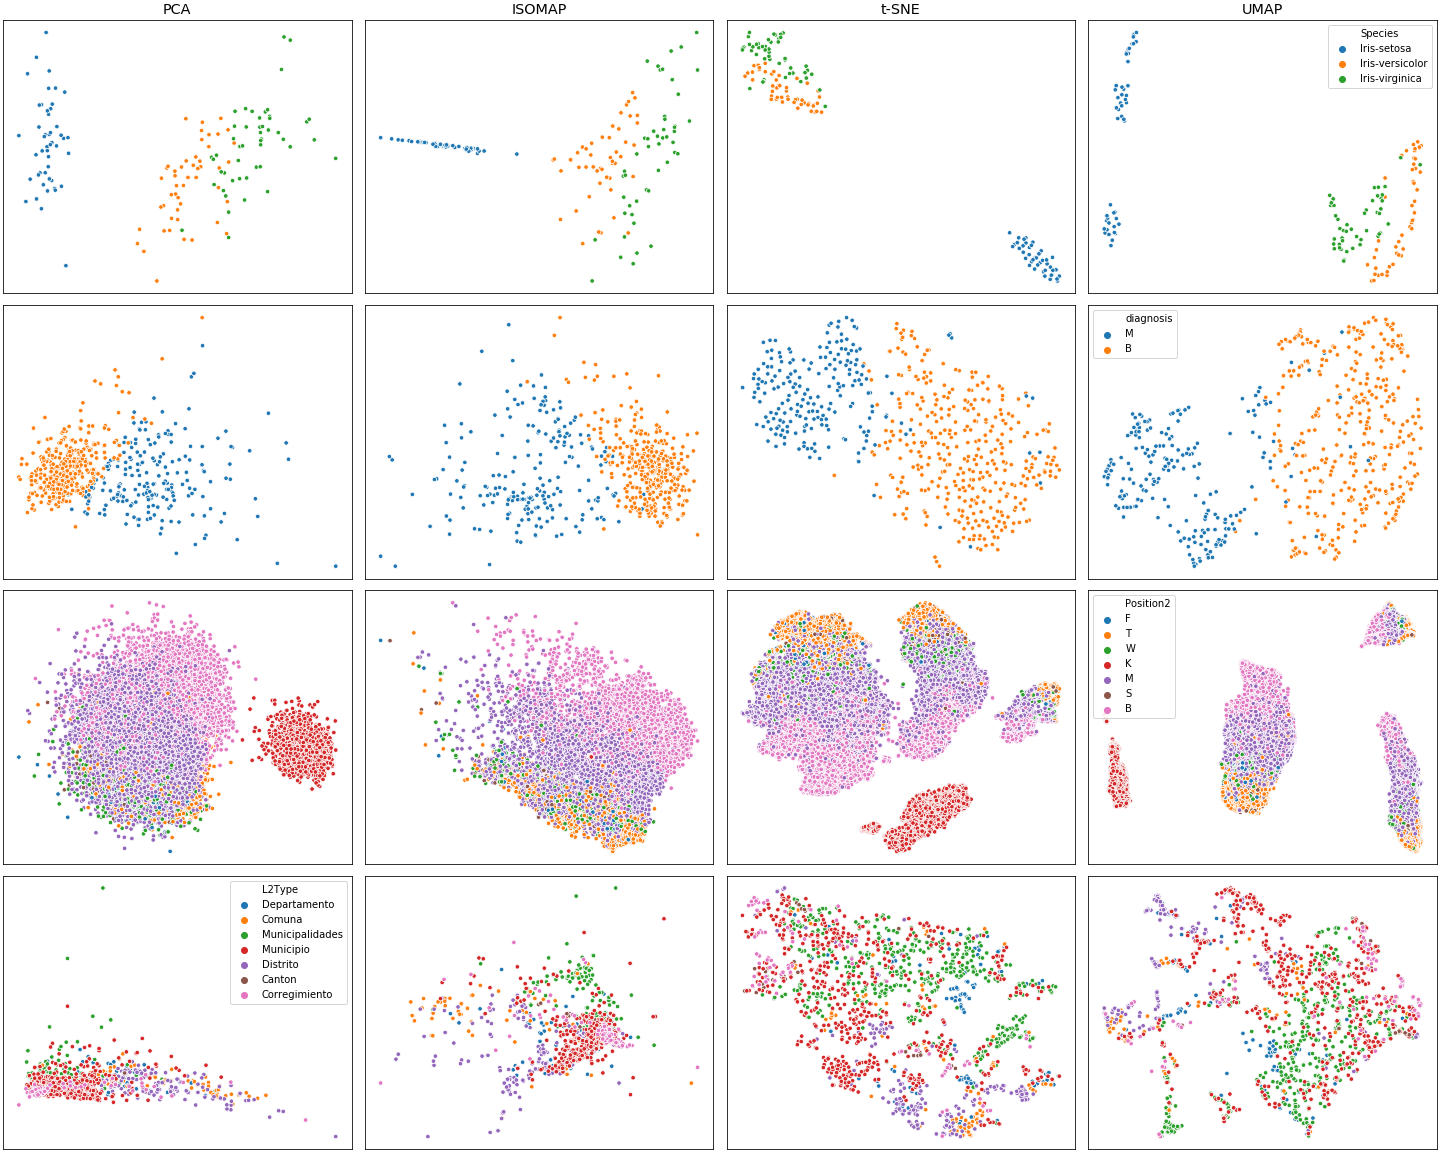
\includegraphics[width=0.9\textwidth]{dr-matrix.png}
 \caption{DR embeddings for 4 datasets: the Iris dataset, the Breast Cancer dataset, the FIFA dataset and the SALURBAL dataset.}
 \label{fig:dr-matrix}
\end{figure}

As appreciate, PCA and ISOMAP tend to overlap the classes making difficult for user to   

\section{Clustering Data}
\label{section3.2}

K-Means
Spectral
Agglomerative
DBSCAN

\section{Interactive DR and Clustering Tools for EDA}
\label{section3.3}

Many researchers have proposed to integrate ML in systems or tools for analyzing data. In \cite{Endert2017b}, a wide range of works are presented and some challenges and opportunities are presented including: (1) incorporation of user feedback, (2) balance human and machine efforts, responsibility and tasks, (3) control of system complexity, (4) visualization of intermediate results, and (5) interpretability. In the context of DR and Clustering, \cite{Wenskovitch2018} and \cite{Sacha2017g} derive from literature review the user tasks and interaction mechanisms incorporated in this kind of systems:

\begin{itemize}
\item DR: See distribution of instances, identify clusters, rotate the embedding, reposition instances, measure distances between instances, change distance metric, select different attributes, modify the weight of an attribute, obtain attribute values and select the algorithm and modify its hyper-parameters.
\item Clustering: Determine cluster structure, label / annotate clusters, merge or split clusters, reposition instances, select different attributes, modify the weight of an attribute, obtain attribute values and select the algorithm and modify its hyper-parameters.
\end{itemize}

A first group of works to denote are 